%!TEX root = ../template.tex
%%%%%%%%%%%%%%%%%%%%%%%%%%%%%%%%%%%%%%%%%%%%%%%%%%%%%%%%%%%%%%%%%%%%
%% chapter2.tex
%% NOVA thesis document file
%%
%% Chapter with research context
%%%%%%%%%%%%%%%%%%%%%%%%%%%%%%%%%%%%%%%%%%%%%%%%%%%%%%%%%%%%%%%%%%%%

%%-------------------------------------------------------------------
%%	2 - Related Work
%%-------------------------------------------------------------------
\chapter{Research Context}
\label{cha:research_context}

% TODO Cap2 - Rever frase AND OR 
The focal point of this dissertation is the implementation of a scalable and coherent distributed data store on top of a set of local (and independent) file systems. The file systems, however, are not used for "general purpose" work: in our deployment, they store VMs - (1) their read-only base images (or templates) and / or (2) their running instances backstores and / or (3) their "support files" (VM specifications, NVRAM / BIOS images, etc).
Furthermore, the target file systems are those which are able to natively provide snapshots and, for the purpose of this dissertation our choice was BTRFS.


 %challenges of implementing a distributed system based on a file system, that can store \textit{VMs} images while leveraging the benefits of snapshots and caching techniques.
 
 Moreover, our work should integrate smoothly into a broader infrastructure illustrated in detail in Section \ref{cha:icbd}.
In this chapter, we start with a survey of core concepts directly associated with the thesis and compliment with some analysis on the state-of-art in the relevant fields.

The organisation of this chapter is as follows:

\begin{description}
	\item [Section~\ref{sec:res_virtualisation}] overviews virtualisation as a core concept, describing significant properties and the inner works of hypervisors and finishes with a comprehensive discussion about the multiple VDI models.
	%
	\item [Section~\ref{sec:res_storage}] studies the principal challenges for a storage system in a VDI context and makes a survey of the multiple types of file systems which are currently prevalent in a data centre environment. 
	%
	\item [Section~\ref{sec:res_caching}] talks about the problem of the locality of the data, and how that fact can influence the performance and scalability of a system.
	%
	\item [Section~\ref{sec:res_replication}] expands on the fact the storing data in a single location is not enough for compliance with current requirements, such as high availability, fault tolerance and performance standards in critical systems.
\end{description}

%%-------------------------------------------------------------------
%%	2.1 - Virtualisation
%%-------------------------------------------------------------------
\section{Virtualisation}
\label{sec:res_virtualisation}

Most of today's machines have such a level of performance that allows the simultaneous execution of multiple applications and the sharing of these resources by several users. In this sense, it is natural to have a line of thought in which all available resources are taken advantage of efficiently. % TODO Refazer este paragrafo

Virtualisation is a technique that allows for the abstraction of the hardware layer and provides the ability to run multiple workloads on a shared set of resources. Nowadays, virtualisation is an integral part of many \textit{IT} sectors with applications ranging from hardware-level virtualisation, operating system-level virtualisation, and high-level language virtual machines.
\nocite{VMware_VM2006}

A Virtual Machine, by design, is an efficient, isolated duplicate of a real machine~\cite{Popek1974}, and therefore should be able to virtualise all hardware resources, including processors, memory, storage, and network connectivity.

For the effort of managing the VMs, there is a need for a software layer that has specific characteristics. One of them is the capability to provide an environment in which VMs conduct operations, acting both as a controller and a translator between the VM and the hardware for all \textit{IO} operations. This piece of software is known as a \gls{VMM}.

In today's architectures, a modern term was been coined, the \textit{Hypervisor}. It is common to mix both concepts (\textit{VMMs} and \textit{Hypervisors}), as being the same, but in fact, there are some details that make them not synonymous.~\cite{Agesen2010}

%%-------------------------------------------------------------------
%%	2.1.X - Hypervisors
%%-------------------------------------------------------------------
\subsection{Hypervisors} % (fold)
\label{sub:res_hypervisors}

The most important aspect of running a VM is that it must provide the illusion of being a real machine, allowing to boot and install any Operating System (OS) available for the real hardware. It is the VMM which has that task and should do it efficiently at the same time providing this three properties~\cite{Popek1974}:

\begin{description}
	\item[Fidelity:] a program should behave on a VM the same way or in much the same way as if it were running on a physical machine.
	%
	\item[Performance:] the vast majority of the instructions in the virtual machine should be executed directly by the real processor without any intervention by the hypervisor.
	%
	\item[Isolation:] the VMM must have complete control over the resources. 
\end{description}

A hypervisor is, therefore, both an Operating System and a Virtual Machine Monitor. It can be deployed on top of a standard OS, such as \textit{Linux} or \textit{Microsoft Windows}, or in a bare metal server.

To start a VM, the hypervisor kernel spins up a VMM, which holds the responsibility of virtualising the architecture and provide the platform where the VM will lie. Thus, since the VM executes on top of the VMM, there is a layer of separation between the VM and the hypervisor kernel, with the necessary calls and data communications taking place through the VMM. This feature confers the necessary degree of isolation to the system. With the hypervisor  kernel taking care of host-centric tasks such as \textit{CPU} and memory scheduling, and network and storage data movement, the VMM assumes responsibility to provide those resources to the VM.

An hypervisor can be classified into two different types~\cite{Aneja2011}, depicting two virtualisation design strategies, as shown in Figure~\ref{fig:hypervisors}:

\begin{figure}[htbp]
	\centering
	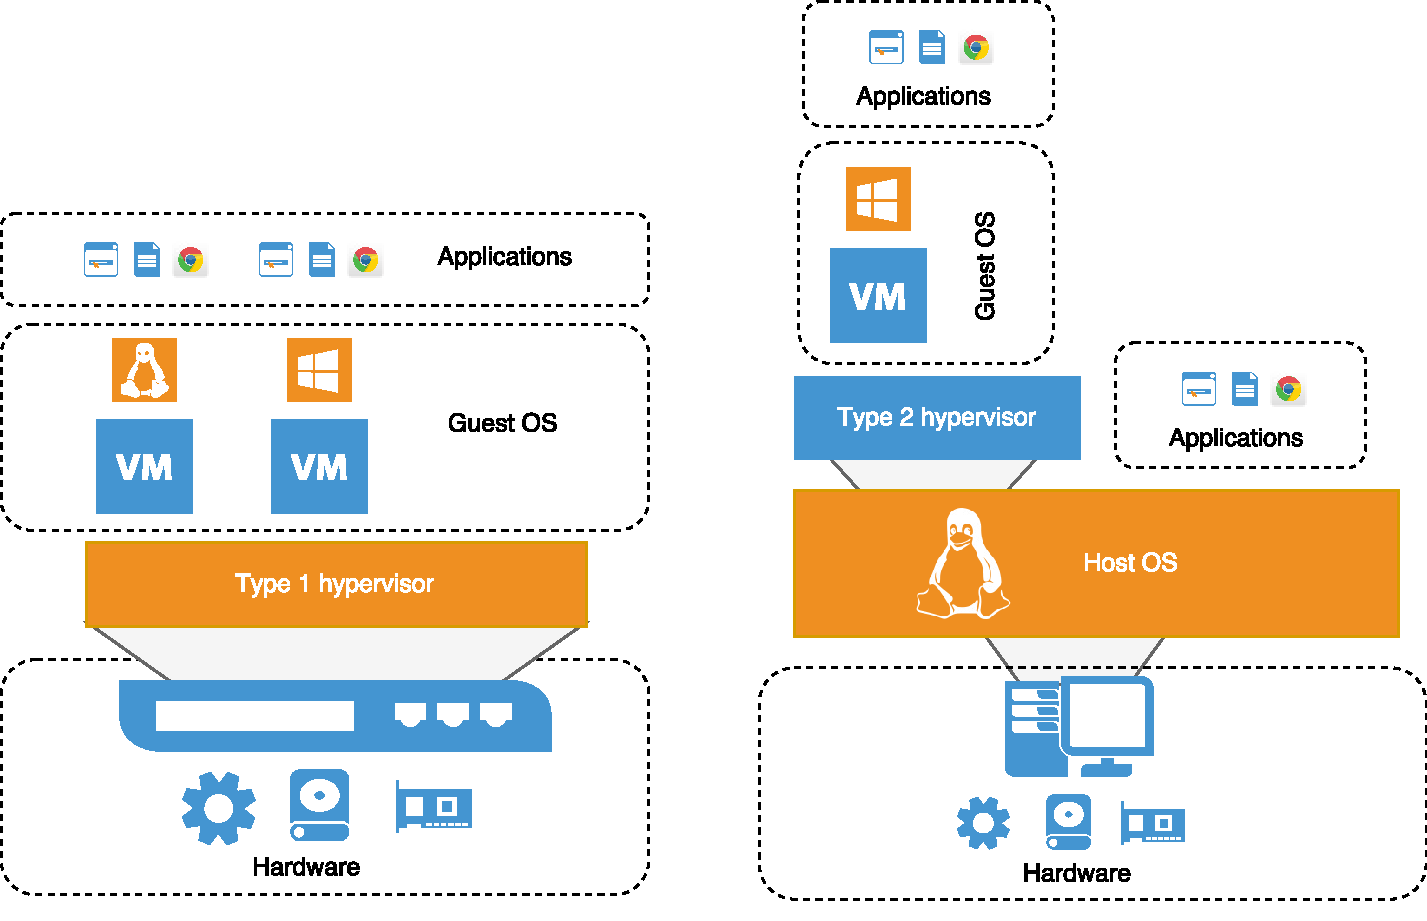
\includegraphics[height=4in]{cap2_hypervisorsv2}
	\caption{Virtualization architecture with type 1 and type 2 hypervisors}
	\label{fig:hypervisors}
\end{figure}

\begin{description}
	\item [Type 1 hypervisor:] Sometimes referred as a bare-metal hypervisor, since there is no need to rely on a host operating system, as it runs directly on the hardware. Moreover, it is the only program executed by the CPU in its most privileged mode. As there isn't any layer between the hypervisor and the resources, this type of hypervisor presents a more efficient solution than the Type 2.

	In addition to the improved performance provided by the sharing or partitioning of devices between the several guest VMs, this architecture provides the benefit of supporting the execution of real-time OSs. The low-level nature of these hypervisors with the broad access to the hardware has proven useful for use-cases that need to deploy a multiplicity of operating systems even in mission-critical circumstances.
	
	Recognising all the facts above, we can point that there are also some disadvantages. Any drivers needed to support different hardware platforms must be covered by the hypervisor package. % TODO Acrescentar o facto de para ter garantias tem que se ter hardware aprovado pelo hypervisor
	
	%Furthermore, considering that Type 1 hypervisors do not have an underlying OS, the complexity of installing and configuring this type of solution increases.
	%
	\item [Type 2 hypervisor:] This second variant of the hypervisor model relies on an already installed operating system and acts very similarly to any conventional process. Here, the hypervisor layer is a union of a host operating system with specialised virtualisation software, including extensions to that OS kernel, that will manage the guest VM. In this case, the hypervisor makes use of the services provided by the OS, which leads to a more significant memory footprint when compared to Type 1 but is integrated seamlessly with the remainder of the system. An excellent illustration of this kind of paradigm is Oracle VirtualBox and VMware Workstation/Fusion~\cite{Agesen2010}.
	
	In this architecture, the host operating system retains ownership of the physical components, with each VM having access to a confined subset of those devices, and the virtual machine monitor providing an environment that emulates the actual hardware per VM. 
	%One advantage is quickness of installation and configuration since the installation process for most of these type of hypervisors only requires the execution of an elemental installer, delivering the instantaneous ability to run a multitude of different operating systems.
	
	All the above culminates in some advantages: Type 2 hypervisors are regularly deployed on desktop an laptop class of hosts, allowing: simulation of a rather complex testing virtualised systems without the expense and complexity of managing dedicated hardware; seamless integration with a graphical environment; host-guest file and print sharing.
	%Also, provide support for running multiple OSs on the same physical machine, which can be valuable for those who rely on multiple applications written for a particular or legacy OS.
\end{description}

Either way, the challenge lays in the fact that the hypervisor needs to provide to guest OS a safe execution environment and at the same time create different machine configurations to each one of them. These characteristics, such as the number and architecture of virtual CPUs (vCPU), the amount and type of memory available (vRAM), the allowed space to store files (vDisk), and so on, are user configurable but it is the job of the hypervisor to do all the resource management. The settings of these individual components reside in a VM configuration file. In the case of VMware hypervisors, the file has the \texttt{.vmx} extension,\cite{VMWare_VMFiles,Portnoy2012} while in a KVM environment, that configuration is stored in a \texttt{.xml} file.~\cite{chirammal2016}

With a virtualised infrastructure there is an opportunity for a substantial reduction in the number of servers which, in turn, diminishes the setup time as those VMs are, in a broad manner, created simply by cloning techniques. Software updates can be hugely simplified and made available to all VMs at once if those VMs are created on-demand from up-to-date templates at the beginning of a user session.
%Even availability is improved since it is an easy task to launch a new VM from a template and migrate all the services that were being made reachable by one that suffered a failure.

% subsection hypervisors (end)

% TODO Cap2 - FICAMOS AQUI NA REVISAO

%%-------------------------------------------------------------------
%%	2.1.X - VDI
%%-------------------------------------------------------------------
\subsection{Virtual Desktop Infrastructure} % (fold)
\label{sub:res_vdi}

\begin{figure}[htbp]
	\centering
	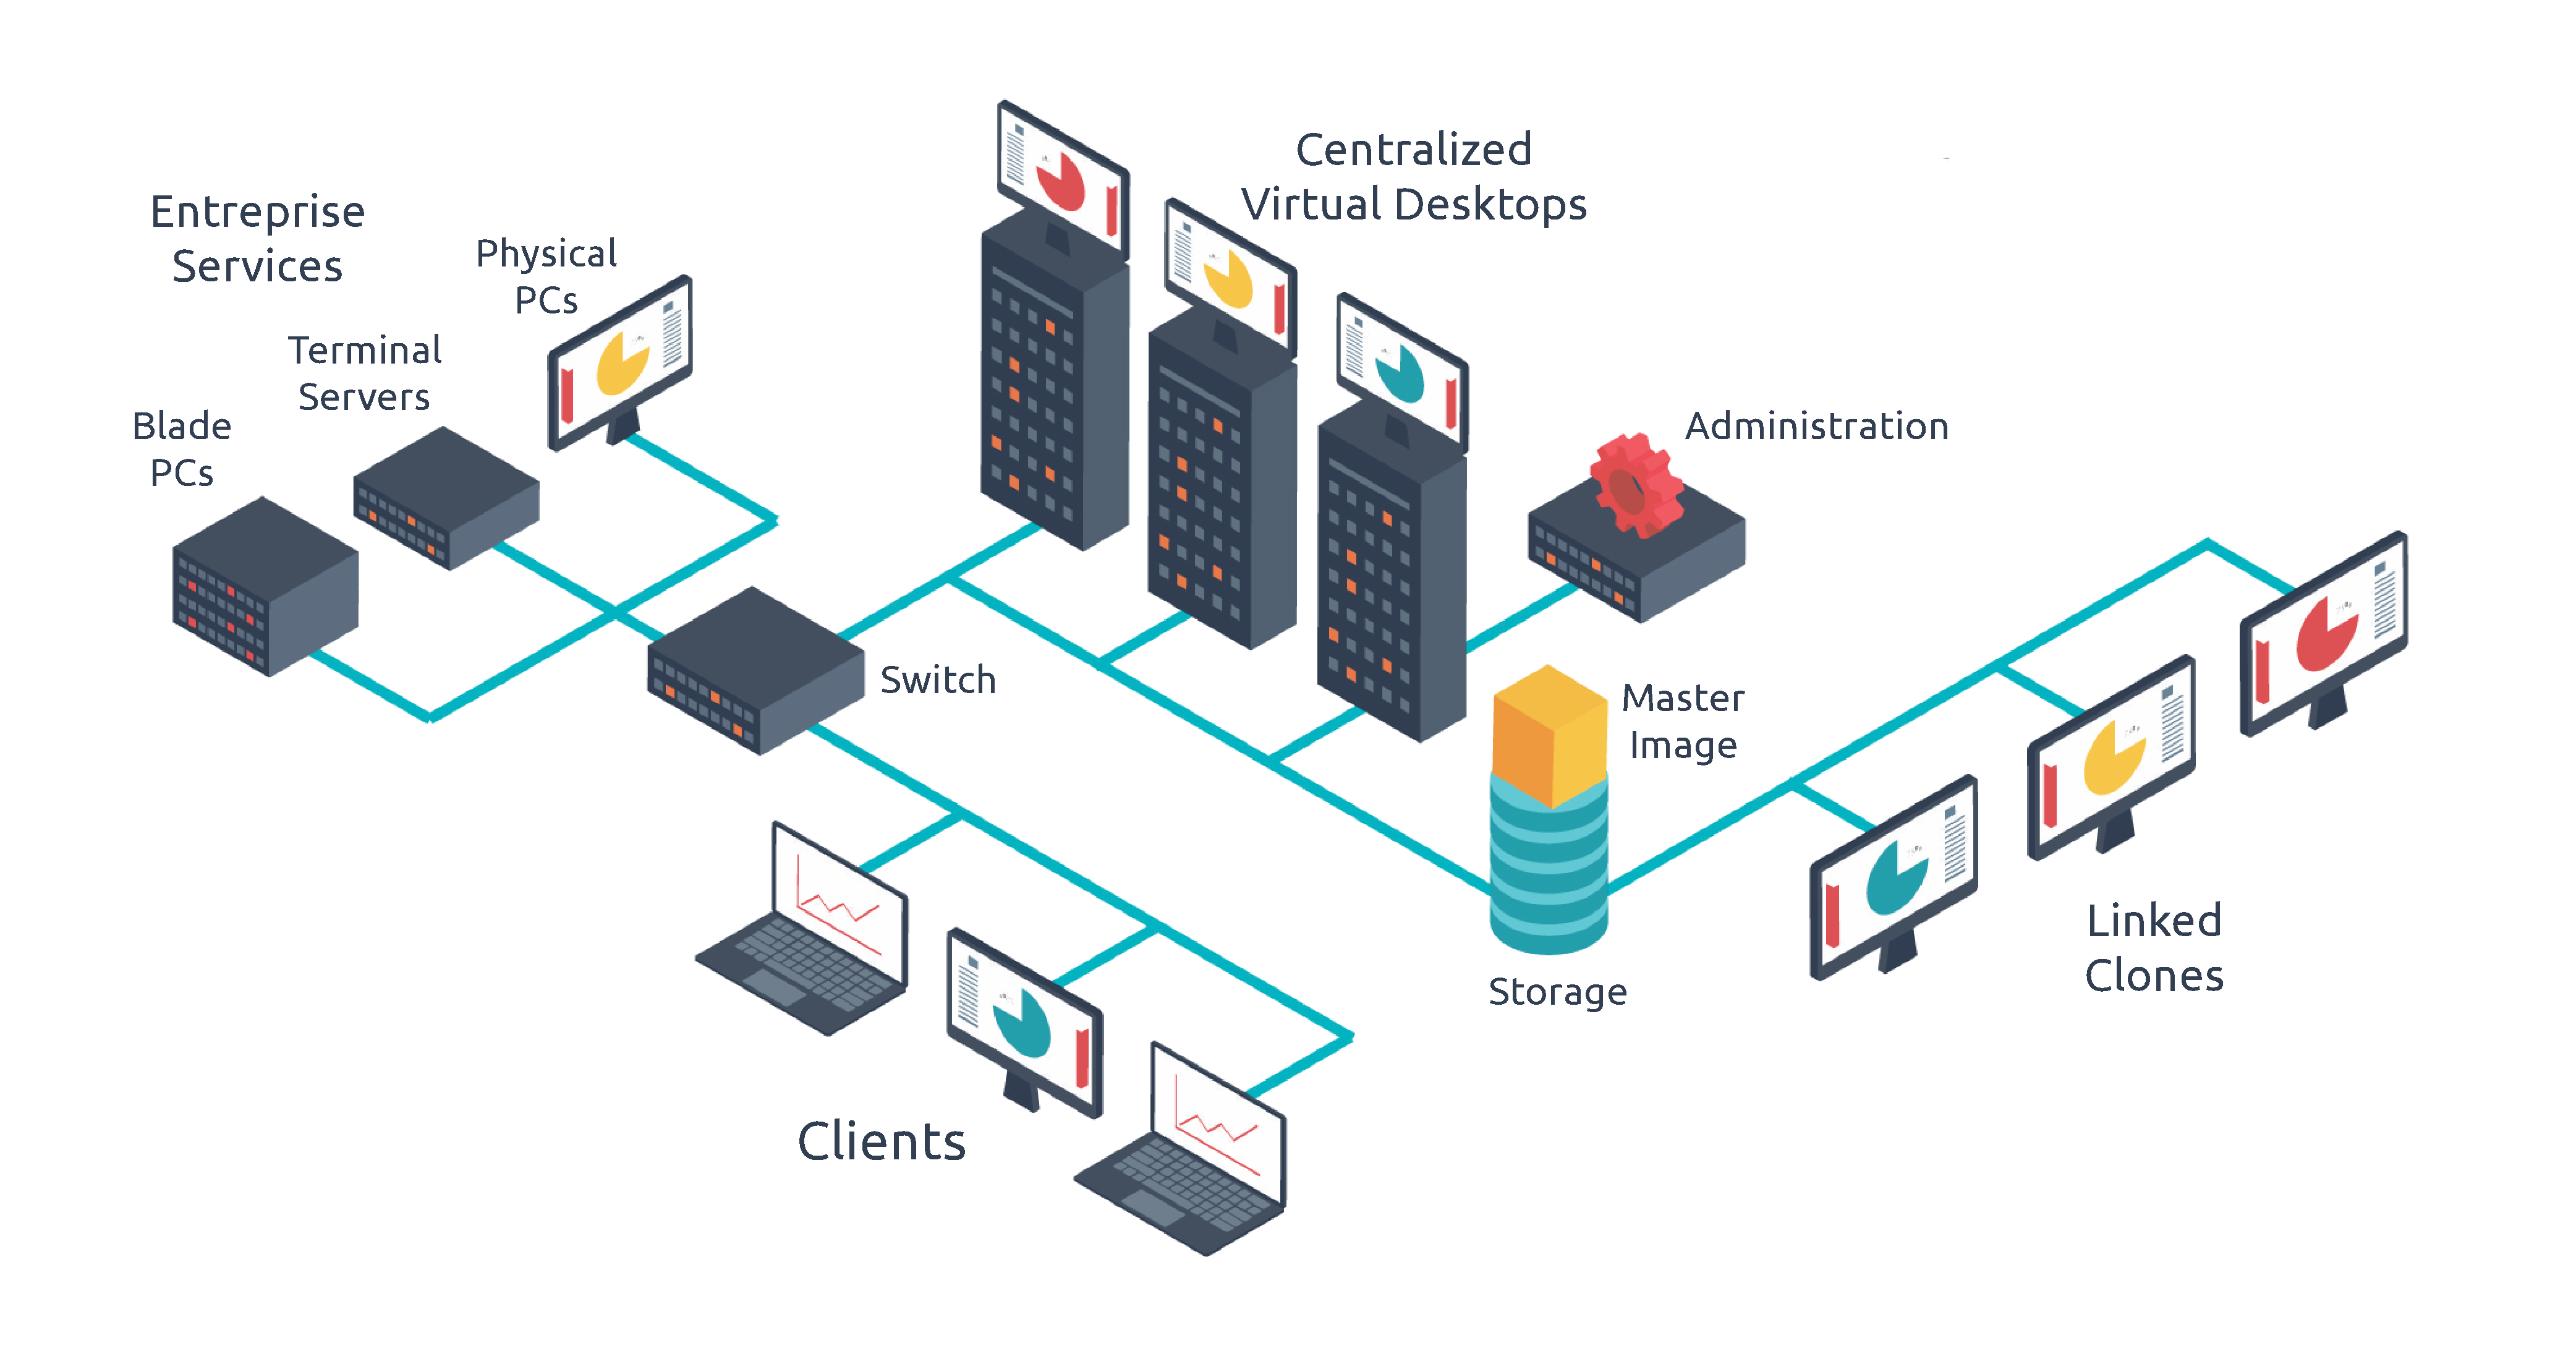
\includegraphics[height=3in]{cap2_VDIv2}
	\caption{An exemple of a Virtual Desktop Infrastructure, adapted from AppDS~\cite{appds_2017}}
	\label{fig:VDI}
\end{figure}

It is common to find in a typical midsize corporate infrastructure hundreds of servers and thousands of workstations. All in a diverse ecosystem counting with many hardware configurations, different OSs and applications needs. Probably even supporting several versions of the same software is required for the day to day operations.

Organisations struggle daily with the traditional problem of installing software in local workstations disks one-by-one (even if employing an automated process). This task tends to be daunting as a company escalates in size and leads to some other predicaments:

\begin{itemize}
	\item A Systems Administrator and IT Staff burden with significant infrastructure administration responsibilities and technical skills.
	%
	\item A delay on the installation or reinstallation of new software and recovery from breakdowns or administration mistakes, which in large installations such intervention could take days.
	%
	\item Installation processes may consume much of the available bandwidth in a network, so if this job is to be executed simultaneously on several workstations, it tends to be scheduled to off work hours to avoid disturbances.
	%
	\item Periodical software updates (such Microsoft's famous Patch Tuesdays~\cite{patch_2017}) are ordinarily released in the morning's first boot of a workstation, which can bloat the traffic and render useless the workstation for the remainder of the update period.
	%
	\item If an update proves to be undesirable, by introducing some unexpected behaviour, it is quite difficult to reverse this situation, which may even demand a new configuration infrastructure-wise.
\end{itemize}

One solution to the unpleasant situations outlined above is to minimise the footprint of installed software and reduce its managing needs. It is possible to conceive all the software required to run a workstation (Operating System and applications) packaged in a single unit like a Virtual Machine. This mechanism allows for the virtualisation of a workstation that can be executed either locally on a typical PC / Laptop, or on a server. The most relevant approach and with more expression at the moment is the \gls{VDI}.

The concept encompasses a series of techniques, providing on-demand availability of desktops, in which, all computing is performed employing virtual machines~\cite{VMWare_VDI2006}.
Typically this solution offers a centralised architecture, where users desktops run in VMs, the user's environment resides on a server in a data centre, as shown in Figure~\ref{fig:VDI}. However, other components are required, such as storage for the users and VMs data and a network capable of moving large data blocks quickly, all in a perspective where from the user's viewpoint there can't be any apparent difference between a virtual desktop and a local installation.

There are two antagonistic approaches to the architecture, one focused on the server-side and the other on the client-side but both solutions are in an in-house paradigm were all configurations, management and storage needs are the responsibility of the business IT staff. A third approach emerged in recent years, with the peculiarity of being cloud-based, coined Desktop as a Service.
In this section, we present a summary of the technologies above-mentioned.

\begin{description}
	\item [Server-based VDI] This is the most common approach, in which the VM runs remotely on a server through a hypervisor. In this model, the images for the virtualised desktops remain deposited in a storage system within a Data Centre. Then, when the times comes for the execution of such VM, a server that is running a hypervisor provisions the VM from storage and puts it into action. Featuring such benefit, as the fact that only a low-performance thin client with support for a protocol such as Remote Desktop Protocol (RDP)~\cite{Microsoft_RDP} or the Remote Framebuffer Protocol (RFB)~\cite{rfc6143} is required to interact with the virtual desktop.

        The downside involves the costs necessary to maintain the service. Highly capable support infrastructure is needed (computing, storage, networking and power). With the additional requirement, of a need in some use cases, for adding high-end graphics processors to satisfy the workflow of customers using multimedia tools. We can still observe that the totality of the computing capacity of the hardware already present in the premises of a client prevails not harnessed. Of course, the machines already present can continue to be used, since they naturally have the resources to use the tools mentioned above, but the non-use of their full potential makes for all past investment made in hardware that pointless.

        There are plenty of commercial solutions that use this principle, with the three most significant players being VMware's Horizon platform~\cite{VMware_horizon}, XenDesktop from Citrix~\cite{Citrix_XenDesktop} and Microsoft with Microsoft Remote Desktop~\cite{Microsoft_RDS}.
	%
	\item [Client-based VDI] In this model, the VM that contains the virtual desktop is executed directly on the client's workstation. This machine makes use of a hypervisor that will wholly handle the virtual desktop.

		Since all computing work predominates on the client side, the support infrastructure (as far as servers are concerned) in this model as a much smaller footprint, having only as a general task to provide a storage environment. Alternatively, all the data could be already locally present in the hard drives of the clients, almost disowning the servers to sheer administration roles and the maintenance of other services.

		The advantages remain close to the previous solution, with the added benefit of a reduced need for resources and the possibility of using some already present in the infrastructure. Although this approach presents itself as significantly more cost restrained, there isn't a notable adoption by software houses in developing products in this family. Reasons for this fact can be attributed to the implementation of such solutions that required a more complicated process, sometimes claiming the complete destruction of locally stored data on workstation hard disks.~\cite{VMblog_Citrix}. An example is a previously existing solution by Citrix, the XenClient~\cite{Citrix_XenDesktop}
	%
	\item [Desktop as a Service] The third, and most modern, concept incorporate the VDI architecture with the made fashionable cloud services. In some aspects shows some astonishing similarities to the server-based method, where servers drive the computation, but here, the infrastructure, the resources and the management efforts are located in the midst of a public cloud.

		The points in favour are some: There is good potential for cost reduction in the field of purchase and maintenance of infrastructure since those charges are imposed on third parties. Every subject related to data security is also in the hands of the platform providers. Enables what is called zero clients, an ultrathin client, typically in a small box form factor, which the only purpose is to connect the required peripherals and rendering pixels onto the user’s display.~\cite{VMWare_Zikmund2014} With the added benefit of presenting very competitive costs per workstation when compared to other types of clients (thick and thin clients) and a reasonable saving on energetic resources.

		However, in contrast, the downsides are also a few. Since the data location frequently is in a place elsewhere from its consumption, some bandwidth problems can arise, limiting the ability to handle a large number of connections. Adding to this mix is the issue of the unavoidable latency, a result of the finite propagation speed of data, which tends to escalate with the distance required to advance. Also, there is the jitter factor, caused by latency variations, which are observed when connections need to travel great lengths through multiple providers with different congestion rates. All these facts not only may lead to a cap on the numbers of clients that are able of connecting simultaneously but also can be a motive in a diminished experience and quality of service provided, when in comparison to the previously presented solutions.
		
		\begin{figure}[htbp]
			\centering
			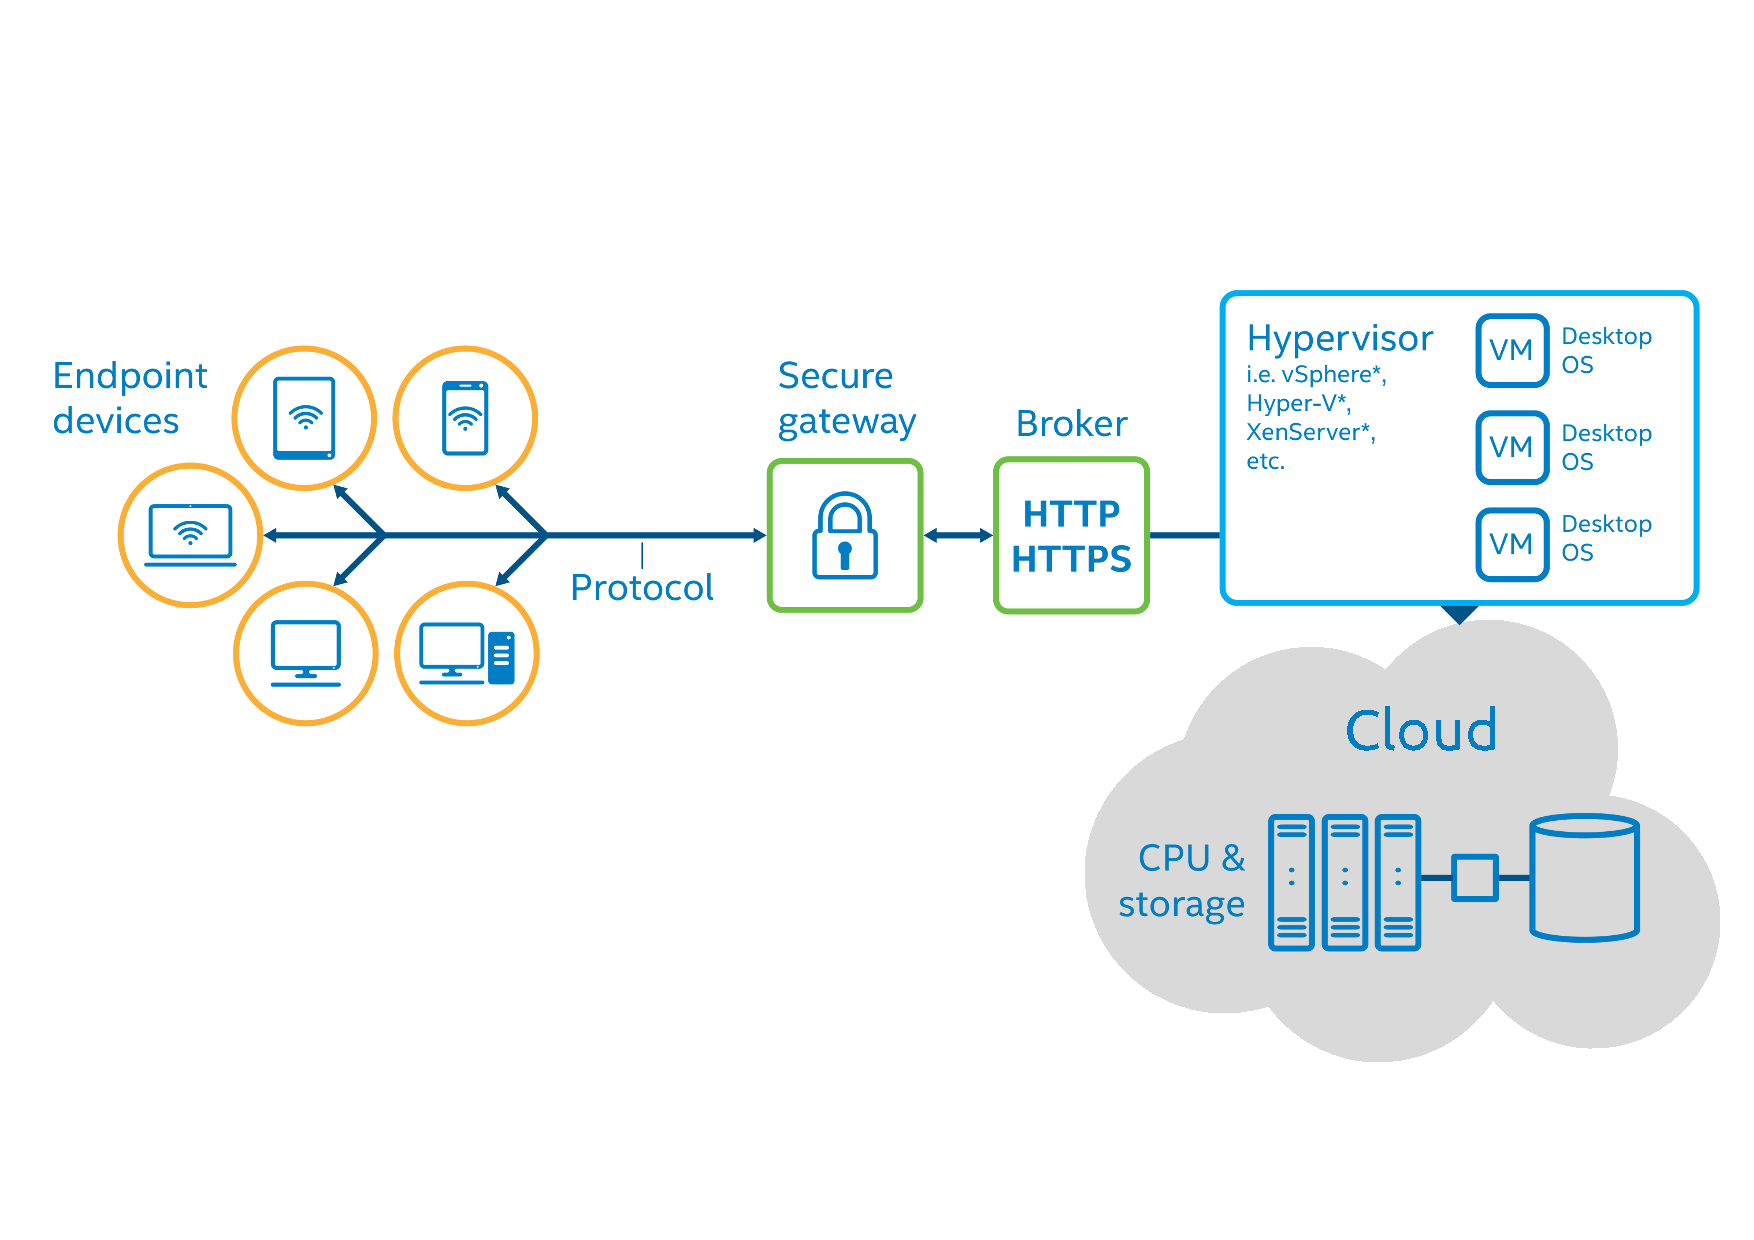
\includegraphics[width=\textwidth]{cap2_daas}
			\caption{Conceptual overview of DaaS architecture, adapted from Intel~\cite{Jain2014}}
			\label{fig:daas}
		\end{figure}

		In this new field, a multitude of solutions is emerging with public cloud providers leading the way. Amazon in its AWS portfolio delivers Amazon Workspaces~\cite{aws_workspaces}, and Microsoft implements the RDS features~\cite{azure_rds} on the Azure product line. Nevertheless, there are also some smaller contenders, as an example, Workspot~\cite{workspot} (a company founded by ex-Citrix employees) makes use of the Microsoft Azure Cloud to provide there take on cloud-native Virtual Desktops.
\end{description}


%\begin{table}[]
%\centering
%\resizebox{\textwidth}{!}{%
%\begin{tabular}{ll}
%                                  & \textbf{Client-Based VDI}                                        	\\
%\textit{\textbf{Deployment}}      & Small server rooms to private data centres                       	\\
%\textit{\textbf{User Experience}} & Should be as good as a local OS installation                     	\\
%\textit{\textbf{Cost}}            & Medium to high in hardware, with some additional cost in software 	\\
%\textit{\textbf{Managing Effort}} & Low                                                               	\\
%\textit{\textbf{Data Location}}   & Within the organisation                                           
%\end{tabular}%
%}
%\caption{Client-Based VDI Characteristics}
%\label{table:clientVDI}
%\end{table}
%
%\begin{table}[]
%\centering
%\resizebox{\textwidth}{!}{%
%\begin{tabular}{ll}
%                                  & \textbf{Server-Based VDI}                                       \\
%\textit{\textbf{Deployment}}      & Small server rooms to private data centres                      \\
%\textit{\textbf{User Experience}} & Not as seamless some lag should be accounted                    \\
%\textit{\textbf{Cost}}            & High to very high in hardware, and also high in software 		\\
%\textit{\textbf{Managing Effort}} & Low to medium                                                   \\
%\textit{\textbf{Data Location}}   & Within the organisation                                           
%\end{tabular}%
%}
%\caption{Server-Based VDI Characteristics}
%\label{table:serverVDI}
%\end{table}
%
%\begin{table}[]
%\centering
%\resizebox{\textwidth}{!}{%
%\begin{tabular}{ll}
%                                  & \textbf{DaaS}                                   \\
%\textit{\textbf{Deployment}}      & Public Cloud                      				\\
%\textit{\textbf{User Experience}} & Not as seamless some lag should be accounted    \\
%\textit{\textbf{Cost}}            & Mostly low, but depending on the provider 		\\
%\textit{\textbf{Managing Effort}} & Low                                             \\
%\textit{\textbf{Data Location}}   & In the cloud, possibly in another geographic location                                           
%\end{tabular}%
%}
%\caption{DaaS Characteristics}
%\label{table:daas}
%\end{table}

\nocite{Nuno2016}
\nocite{Eduardo2016}
\nocite{P2020}


%%-------------------------------------------------------------------
%%	2.1.X - VM storage
%%-------------------------------------------------------------------
\subsection{Virtual Machine Image Storage} % (fold)
\label{sub:res_vm_storage}

The data storage is one of the focal points to address in this work. Therefore, it is meaningful to understand how a virtual machine is composed and how is translated to a representation in a storage device.

The basic anatomy of a Virtual Machine encompasses a collection of files that define the VM settings, store the data (i.e. Virtual Disks) and save information about the state of its execution. All of these data and metadata need to be deposited on storage devices of whatever type. \\

\textbf{VMware Architecture} \quad Given the architecture presented by VMware software~\cite{VMWare_VMFiles}, the main files required for the operation of a VM are:

\begin{itemize}
    \item \emph{The VM configuration file} - The \texttt{.vmx} file holds the primary configuration options, defining every aspect of the VM. Any virtual hardware assigned to a VM is present here. 
		At the creation time of a new virtual machine, the configurations regarding the guest operating system, disk sizes, and networking are appended to the \texttt{.vmx} file. Also, whenever an edit occurs to the settings of a virtual machine, this file is updated to reflect those modifications.
	%
    \item \emph{The virtual disk files} - Embodying multiple \texttt{.vmdk}, which stores the contents of the virtual machine's hard disk drive and a small text disk descriptor file.
		The descriptor file specifies the size and geometry of the virtual disk file. Also includes a pointer to the full data file as well as information regarding the virtual disks drive sectors, heads, cylinders and disk adapter type.
		The virtual disk actual data file is conceived while adding a virtual hard drive to a VM. The size of these files will fluctuate based on the maximum size of the disk, and the type of provisioning employed (i.e. thick or thin provisioning)
    %
    \item \emph{The file that stores the BIOS} - The \texttt{.nvram} file stores the state of the virtual machine's BIOS.
    %
    \item \emph{The suspended state file} - The \texttt{.vmss} saves contains the state of a suspended virtual machine. This file is utilised when virtual machines enter a suspended state giving the functionality of preserving the memory contents of a running VM so it can start up again where it left off.  When a VM is returned from a suspend state, the contents of this file are rewritten into the physical memory of the host, being deleted in the event of the next VM Poweroff.
    %
    \item \emph{Log files} - A collection of \texttt{.log} files is created to log information about the virtual machine and often handled for troubleshooting purposes. A new log file is created either during a VM power off and back on process, or if the log file stretches to the maximum designated size limit.
	%
	\item \emph{The Swap file} - The \texttt{vswp} file warehouses the memory overflow in case  the host cannot provide sufficient memory to the VM, and Ballooning technique cannot be employed to free memory~\cite{VMWare_esxmem} 
\end{itemize}

In addition to the records described above, there may be some more files associated with the use of snapshots. More concretely, a \texttt{.vmsd} file and multiple \texttt{.vmsn}. The first is a file with the consolidation of storing and metadata information about snapshots. The other one, represents the snapshot itself, saving the state of the virtual machine in the moment of the creation of the snapshot.

The implementation of snapshots mentioned above applies to a specific implementation of VMware and takes form as follows: first, the state of the resource is stored in the form of an immutable and persistent object. Then, all modifications that transform the state of the resource are gathered in a different object. 
The diverse snapshotting techniques are addressed in a more comprehensive sense in the Section~\ref{sub:res_snapshots}.


%%-------------------------------------------------------------------
%%	2.2 - Storage
%%-------------------------------------------------------------------
\section{Storage} % (fold)
\label{sec:res_storage}

As stated in previous sections, the main problem to be addressed in this work is the storage concerning virtual machines. That could be either images, snapshots, files or data structures that are needed to support the execution of a VM. 

When applied to the VDI concept some demands appear in the form of specific care needed at planning the storage system architecture, as well as the supporting infrastructure: the hardware picked, network topology, protocols used, and software implemented.

At the end of the day, the idea is to present a solution that offers an appropriate cost to performance ratio, and that with little effort can scale when the need emerges.


%%-------------------------------------------------------------------
%%	2.2. - Storage Challenges
%%-------------------------------------------------------------------
\subsection{Storage Challenges}
\label{sub:res_storage_challenges}

In a typical data centre application, with a well-designed infrastructure and in normal conditions, the storage system is steadily used but isn't being stressed continuously with requests I/O requests that directly affect the system performance. However, that postulate is no longer valid when talking about the storing of VM files for use in a VDI environment. In this type of context, some events can cascade in I/O storms that eventually introduce degradations in storage response time, which diminishes the performance of the overall system and in turn leads to a lower satisfaction level for the users of said system.

\paragraph{I/O Storms}
\label{par:res_ios_storms}

In a typical data centre application, with a well-designed infrastructure and in normal conditions, the storage system is steadily used but isn't being stressed continuously with I/O requests that directly affect the system performance. However, that postulate is no longer valid when talking about the storing of VM files for use in a VDI environment. In this type of context, some events can cascade in I/O storms that eventually introduce degradations in storage response time, which diminishes the performance of the overall system and in turn leads to a lower satisfaction level for the users of said system.
From several events that influence a storage system we can point out some that have more expression in a VDI setting:

\begin{description}
	\item [Boot Storm] It may happen, on the occasion of the starting a work shift; with several users simultaneously arriving at their desk and booting their workstations. In this circumstance, all VMs are simultaneously performing multiple read and write operations on the storage system, which translates into poor response times and a long wait for the end of the boot process.
	%
	\item [Login Storm] Right after the booting an OS, the workstations are not entirely operational users have to log in to access a desktop, including applications and files. This procedure, results in a considerable number of concurrent I/O requests from multiple VMs in a short time, as the system attempts to load quite a few files related to the user's profile.
	%
	\item [Malware and Anti-Virus Software Scanning] Usually scans for unwanted files and untrusted applications, are scheduled to execute at a time when they cause the least possible impact taking into consideration the load of the machine. However, it is not uncommon to observe a behaviour where this kind of software starts a scan right after boot. Alternatively, the unfortunate case where different machines decide to start that examination at the same time, causing a negative impact on every machine.
	%
	\item [Big Applications Needs] Some applications can be very I/O intensive, like loading a project in an IDE with numerous libraries and dependencies that need to be reviewed at startup. Also, we can envision a scenario where multiple users simultaneously open the same very resource intensive application, for instance, in a classroom, the teacher asks the students to start a particular application, the I/O requests to the storage system will most likely be simultaneous.
	%
	\item [Operating System Updates] Similarly to Malware and Anti-Virus Software Scanning, the update process of an Operating System will most likely be tied to a schedule that is based on the current load of a machine. Yet, multiple systems may decide to perform an update in the same space of time thus leading to the bottleneck problem of concurrent access to the storage system.
\end{description}

	 
	 


%%-------------------------------------------------------------------
%%	2.2. - File Systems
%%-------------------------------------------------------------------
\subsection{File Systems} % (fold)
\label{sub:res_file_systems}

The traditional and perhaps most common way of storing files and, in turn, VMs is the use of file systems.
This kind of system is used to manage the way information is stored and accessed on storage devices. A file system can be divided into three broad layers, from a top-down perspective we have:

\begin{itemize}
	\item The \textbf{Application Layer} is responsible for mediating the interaction with user's applications, providing an API for file operations. This layer gives file and directory access matching external names adopted by the user to the internal identifiers of the files. Also, manages the metadata necessary to identify each file in the appropriate organisational format.
	%
	\item Then the \textbf{Logic Layer} is engaged in creating a hardware abstraction through the creation of logical volumes resulting from the use of partitions, RAID volumes, LUNs, among others.
	%
	\item The last one is the \textbf{Physical Layer}. This layer is in charge with the physical operations of the storage device, typically a disk. Handling the placement of blocks in specific locations, buffering and memory management.
\end{itemize}


There are many different types of file systems, each one boasting unique features, which can range from security aspects, a regard for scalability or even the structure followed to manage storage space.

\begin{description}
	\item [Local file systems:] A local filesystem can establish and destroy directories, files can be written and read, both can move from place to place in the hierarchy but everything contained within a single computing node. 
		Good performance can be improved in certain ways, incorporating caching techniques, read ahead, and carefully placing the blocks of the same file close to each other, although scalability will always be reduced. 
		There are too many file systems of this genre to be here listed. Nevertheless, some of the most renowned may be mentioned. As the industry-standard File Allocation Table (FAT), the New Technology File System (NTFS) from Microsoft, the Apple's Hierarchical File System Plus (HFS+) also called Mac OS Extended and the B-tree file system (BTRFS) initially designed by Oracle.
	% 
	\item [Distributed file system:] A distributed file system enables access to remote files using the same interfaces and semantics as local files, allowing users to access files from any computer on a network. 
		Distributed file systems are being massively employed in today's model of computing. They offer state-of-the-art implementations that are highly scalable, provide great performance across all kinds of network topologies and recover from failures. 
		Because these file systems carry a level of complexity considerably higher than a local file system, there is a need to define various requirements such being transparent in many forms (access, location, mobility, performance, scaling). As well as, handle file replication, offer consistency and provide some sort of access-control mechanisms. 
		All of these requirements are declared and discussed in more detail in the book \enquote{Distributed Systems: Concepts and Design} by George Coulouris et al.~\cite{Coulouris2011}
		We can give as example of file systems the well-known Network File System (NFS)~\cite{rfc5661} originally developed by Sun Microsystems, and the notable Andrew File System (AFS)~\cite{Satyanarayanan1990} developed at Carnegie Mellon University.
\end{description}

There are numerous types of additional file systems not mentioned since they are not in the domain of this work. Still, it is important to note the existence of an architecture that is not similar to the traditional file hierarchy adopted in file systems, which is the object-based storage. 

This structure, as opposed to the ones presented above, manages data into evenly sized blocks within sectors of the physical disk. It is possible to verify that it has gained traction leading to the advent of the concept of cloud storage. There are numerous implementations of this architecture, whether in small local deployments or large-scale data centres supporting hundreds of petabytes of data.
This type of file system is being studied in the context of a parallel thesis but inserted in the same project already presented.

It is worthwhile to enumerate some examples such as CephFS~\cite{Weil2006}, OpenStack Swift~\cite{Swift2017}, and in a IaaS flavour the Amazon S3~\cite{aws_s3} and Google Cloud Storage~\cite{gcp_storage}.


%%-------------------------------------------------------------------
%%	2.2. - Snapshots
%%-------------------------------------------------------------------
\subsection{Snapshots} % (fold)
\label{sub:res_snapshots}

In this work, the snapshot functionality of the file system itself is a valuable asset. This technique is present in some of the most recently designed file systems, such as the BTRFS. 
As the name implies, a snapshot is an image at a given instant of the state of a resource,  we are particularly interested in snapshots of volumes (logical disks), and of files (individually or grouped, for example, in a directory).

The implementation of a snapshot can be described as follows: a) the state of a resource is saved in the form of a persistent and immutable "object"; b) changes to the state of the resource forces the creation and storage of another object. Consequently, it is possible to return to any previous state, as long as, the object corresponding to that state is available. Snapshots are especially interesting in virtualised environments because the hypervisor can take snapshots of the most critical features of a VM: CPU, memory, and disk(s). 

In this work, we propose to use the snapshot functionality of the file system itself, present in some of the most recently designed file systems, such as the BTRFS. This way the creation of linked-clones is handled by the file system capabilities as an alternative to linked-clones created by virtualisation software itself

In order for multiple snapshots, do not take up space unnecessarily, data compression techniques are applied when implementing snapshots. So, the new object created to register the sequence of new changes of a resource only registers the modifications made, keeping unchanged the state in the initial (parent) object. This phenomenon (i.e. the changes between the current snapshot and the previous one) is called a "delta" connecting snapshots.



%%-------------------------------------------------------------------
%%	2.3. - Caching
%%-------------------------------------------------------------------
\section{Caching} % (fold)
\label{sec:res_caching}

%!!! \textbf{TODO} - Needs More Info!!!
% TODO Cap2 - Caching

A cache can be defined as a store of recently used data objects that is nearby one client or a particular set of clients than the objects themselves. The inner works of one of these systems are rather simple. When a new object is obtained from a server, it is added to the local cache, replacing some existing objects if needed. That way when an object is requested by a client, the caching service first checks the cache and supplies the object from there if an up-to-date copy is available. If not, an up-to-date copy is fetched, then served to the client and stored in the cache. 

Caching often plays a crucial role in the performance and scalability of a file system and is used extensively in practice.

Caches may be found beside each client or they may be located on a server that can be shared by numerous clients.

\begin{description}
	\item [Server-side Cache:] Server side caching is when the caching data occur on the server. There is no right way to the approach of caching data; it can be cached anywhere and at any point on the server assuming it makes sense. It is common to cache frequently used data from a DataBase to prevent connecting to the DB every time some data is requested. In a web context, it is common to cache entire pages or page fragments so that there is no need to generate a web page every single time a visitor arrives.
	%
	\item [Client-side Cache:] Maintaining the analogy to the Web environment, caches are also used on the client side. For instances, Web browsers keep a cache of lately visited web pages and other web resources in the client’s local file system. Then when the time comes to serve a page that is stored in the cache, a special HTTP request is used to check, with the corresponding server, if the cached page is up-to-date. In a positive response the page is simply displayed from the cache, if not, the client just needs to make a normal request.
\end{description}



%%-------------------------------------------------------------------
%%	2.4. - Replication
%%-------------------------------------------------------------------
\section{Replication}
\label{sec:res_replication}

%!!! \textbf{TODO} - Needs More Info!!!
% TODO Cap2 - Replication 

At the storage level, replication is focused on a block of binary data. Replication may be done either on block devices or at the file-system level. In both cases, replication is dealing with unstructured binary data. The variety of technologies for storage-level replication is very extensive, from commodity RAID arrays to network file system.
File-based replication works at a logical level of the storage system rather than replicating at the storage block level. There are multiple different methods of performing this. And, unlike with storage-level replication, these solutions almost exclusively rely on software.

Replication is a key technology for providing high availability and fault tolerance in distributed systems. Nowadays, high availability is of increasing interest with the current tendency towards mobile computing and consequently the appearance of disconnected operation. Fault tolerance is an enduring concern for does who provide services in critical and other important systems.

There are several arguments for which replication techniques are widely adopted; these three are of significant importance:

\begin{description}
	\item [Performance improvement:] Performance improvement: Replication of immutable data is a trivial subject, is nothing more than a copy of data from one place to another. This increases performance, sharing the workload with more machines with little cost within the infrastructure.
	%
	\item [Increased availability:] Replication presents itself as a technique for automatically keeping the availability of data despite server failures. If data is replicated in additional servers, then clients may be able to access that data from the servers that didn't experience a failure.
		Another factors that must be taken into account are network partitions and disconnected operation.
	%
	\item [Fault tolerance:] There is the need o maintain the correctness guarantees of the data in the appearance of failures, which may occur at any time.
\end{description}

% section replication_consistency (end)




 
